\documentclass[11pt]{report}
\usepackage{graphicx}
\usepackage{amsmath}
\title{CS440 Project 1 Report}
\author{Douglas Gromek, Michael Comatas, Xiaoyu Sun}

\begin{document}
\maketitle
\section*{Part 1}
\paragraph{a)}
Explain in your report why the first move of the agent for the example search problem from Figure 8 is to the east rather than the north given that the agent does not know initially which cells are blocked.\\

\begin{figure}[h]
\begin{center}
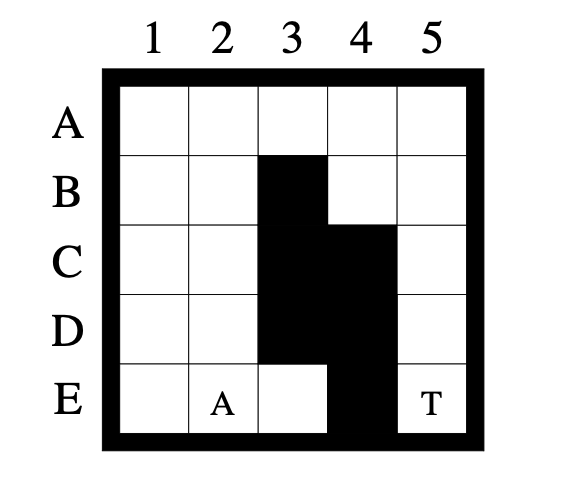
\includegraphics[width=0.3\textwidth]{Part1a_Sample}
\caption{Example Search Problem Initial State}
\end{center}
\end{figure}
\subparagraph{Answer:}
Since the agent does not know initially which cells are blocked. The path planning is solely based on the evaluation function. We know that A* uses f(x) = g(x) + h(x) (cost-to-come + estimated cost-to-go). Here we choose Manhattan distances as h-value; All costs g(x) are one. Also the algorithm will remember the expanded nodes.
At initial state, the neighbors of A(E2) are \{E1, D2, E3\}, the values of each node is denoted by [cost, h-value]. After expanded the root node we got:\\
\begin{center}
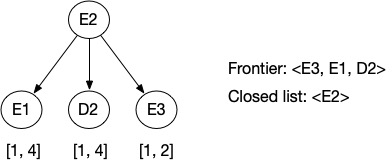
\includegraphics[scale = 0.5]{Part1a_1}
\end{center}

Here we can see that E3 has the smallest f(x) = 1 + 2 = 3. Such that we choose E3 to expand next. From the grid we know that the neighbors of E3 are \{E2, D3, E4\}, since E2 already in the closed list, we would not visit it again. After expanded E3 we got:

\begin{center}
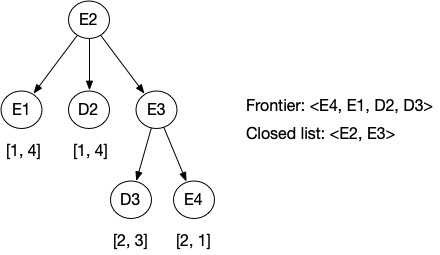
\includegraphics[scale=0.5]{Part1a_2}
\end{center}

Here we can see that E4 has the smallest f(x) = 2 + 1 = 3, such that we next expand E4. Same as above, after we expanded E4 we got:

\begin{center}
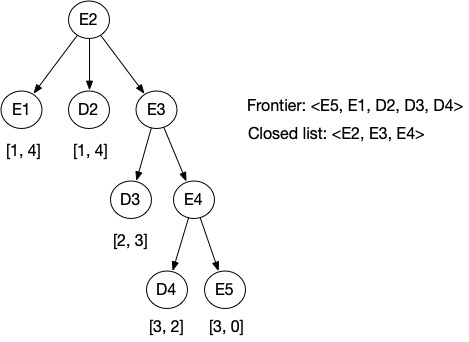
\includegraphics[scale=0.5]{Part1a_3}
\end{center}

Now E5 has the smallest f(x) = 3 + 0 = 3, such that we choose E5 to expand next. While E5 is the goal state, we stop the A* search, then we got the path from the initial state to goal state which is: 

\begin{center}
E2(A) $\rightarrow$ E3 $\rightarrow$ E4 $\rightarrow$ E5(T)
\end{center}
Thus, the first move is to the east. \\
\newpage

\paragraph{b)}
This project argues that the agent is guaranteed to reach the target if it is not separated from it by blocked cells. Give a convincing argument that the agent in finite gridworlds indeed either reaches the target or discovers that this is impossible in finite time. Prove that the number of moves of the agent until it reaches the target or discovers that this is impossible is bounded from above by the number of unblocked cells squared.\\

\subparagraph{Answer:}
Given that the agent is not separated from the target by blocked cells, and the agent in finite gridworlds, one of the possibilities that the algorithm cannot finish the mission is: the agent might be stuck in an infinite loop. Here we use A* to determine the shortest path, and our algorithm would remember the expanded nodes, which prevent us from keeping visit the same node and stuck in an infinite loop. Also, by using repeated A*, the agent will do A* search repeatedly until it reaches the target. Even when the agent encounters a blocked cell that in the current path, it will not be stuck there, but re-planning a new “shortest presumed-unblocked path.” Thus, the agent in finite gridworlds is guaranteed to reach the target if it is not separated from it by blocked cells.

On the other hand, if the agent is separated from the target by blocked cell, the algorithm would discover that this is impossible in finite time. Because it will repeatedly execute the search method and ends up all the possibilities were tried and get the result that it is impossible to solve it in finite time.\\

\textbf{Proof:}\\

\indent Say that there are \textbf{n} unblocked cells in the grid world. Because our A* algorithm would keep the expanded nodes in the closed list, so the path would not visit the same cell again; In the worst case, within one A* process the agent need to expand every unblocked cell other than the goal state to get a result, so the maximum moves the agent can take of each A* is \textbf{m}, $$m < n$$

Moreover, in the worst case, every time the agent moves along the path, it will encounter a blocked cell in current path somewhere, and need to re-implement A*. The maximum number of times A* is called is \textbf{r}, $$r<n$$ because there is no need to implement A* in the target node.

Therefore, in the worst case, since every time we call A*, we will clear the closed list, so it is possible that the agent will traverse the whole unblocked region every time we implement A*, no matter if there is a solution path or not. We know that the total number of moves of an agent =  (the total number of times A* is called) * (total number of moves for each A* call),$$m \times r < n^2$$

Thus, the number of moves of the agent until it discovers that this is impossible is bounded from above by the number of unblocked cells squared. 

Q.E.D.
\newpage

\section*{Part 2}
Repeated Forward A* needs to break ties to decide which cell to expand next if several cells have the same smallest f-value. It can either break ties in favor of cells with smaller g-values or in favor of cells with larger g-values. Implement and compare both versions of Repeated Forward A* with respect to their runtime or, equivalently, number of expanded cells. Explain your observations in detail, that is, explain what you observed and give a reason for the observation.\\

\paragraph{Observation:}

In this part, we implement forward A* with tiebreaker in favor of cells with smaller g-values, and in favor of cells with larger g-values. By comparing their run-times, we can see the differences from the line chart - figure 2. Using larger g-value as tie breaker will takes less runtime, because with larger g-value, we care about smaller h-value, which makes the search become goal-oriented. Instead of search in radial.

\begin{figure}[h]
\begin{center}
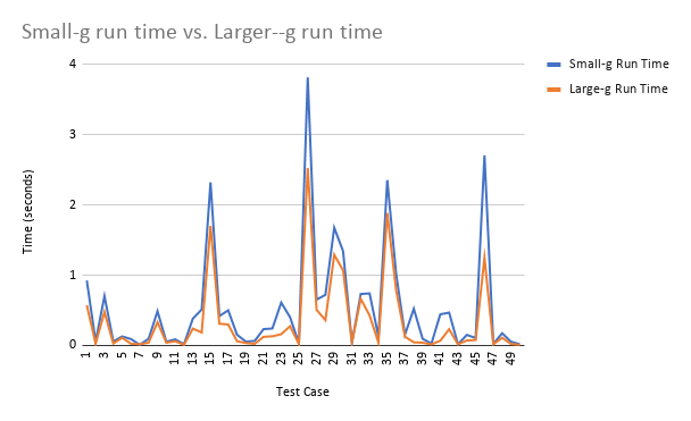
\includegraphics[width = 1\textwidth]{Part2_1.jpg} 
\end{center}
\caption{Comparing lager g-value and smaller g-value}
\end{figure}

\newpage


\paragraph{Explanaiton}
To demonstrate how the A* algorithm breaks ties using smaller g-value, imagine that we have a gridworld like the one in figure 3, where A is the start node and T is the goal node.

We can see that in figure 3, since we are using smaller g-value as a tie-breaker, it will always expand the nodes with smaller g-value, which causes the situation in the image, in this case, it is just like Breadth-First Search.


\begin{figure}[h]
\begin{center}
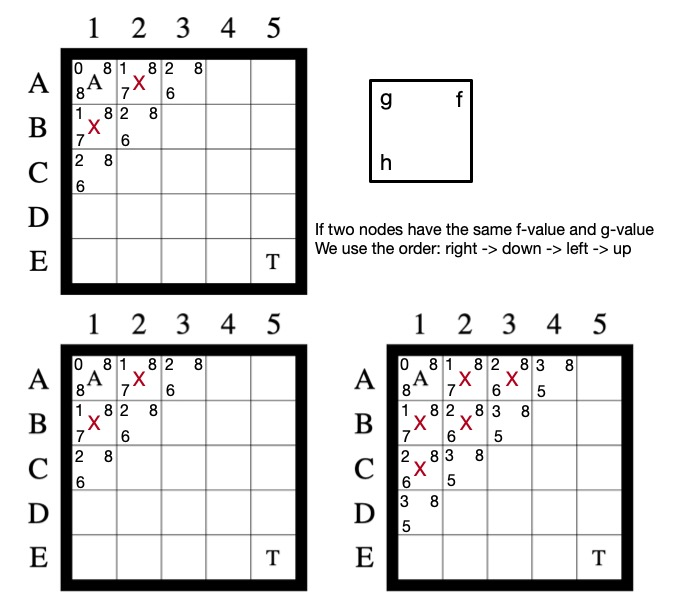
\includegraphics[width = 0.8\textwidth]{Part2_2.jpg} 
\end{center}
\caption{demostrate A* with smaller g-value as tie-breaker}
\end{figure}

\begin{figure}[t]
\begin{center}
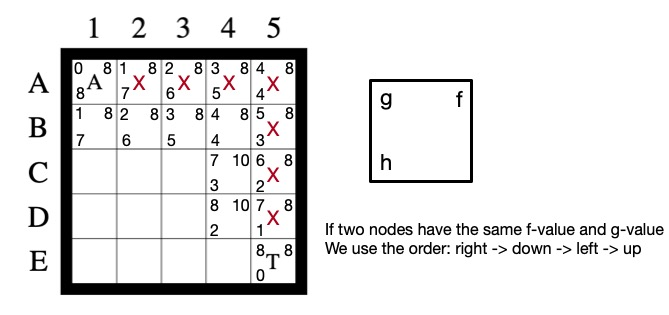
\includegraphics[scale = 0.5]{Part2_3.jpg} 
\end{center}
\caption{demonstrate A* with larger g-value as tie-breaker}
\end{figure}

In figure 4 we see the path the agent will take when tie breaker is based on larger g-values. In this scenario we are always expanding nodes that have taken more steps towards the goal, it makes the search become goal-oriented. This is why using a higher g-value to determine tie breakers is a more efficient method.

\newpage


\section*{Part 3}
Implement and compare Repeated Forward A* and Repeated Backward A* with respect to their runtime or, equivalently, number of expanded cells. Explain your observations in detail, that is, explain what you observed and give a reason for the observation. Both versions of Repeated A* should break ties among cells with the same f-value in favor of cells with larger g-values and remaining ties in an identical way, for example randomly.


\paragraph{Observation:}
Here we implement Repeated Forward A* and Repeated Backward A* with larger-g as tie-breaker. We can see from figure 5, it is hard to say which one is better. In some cases, Backward A* has better performance; In other cases, Forward A* has better performance. The reason is that the advantages of each strategy depend on how the maze looks like.

\begin{figure}[h]
\begin{center}
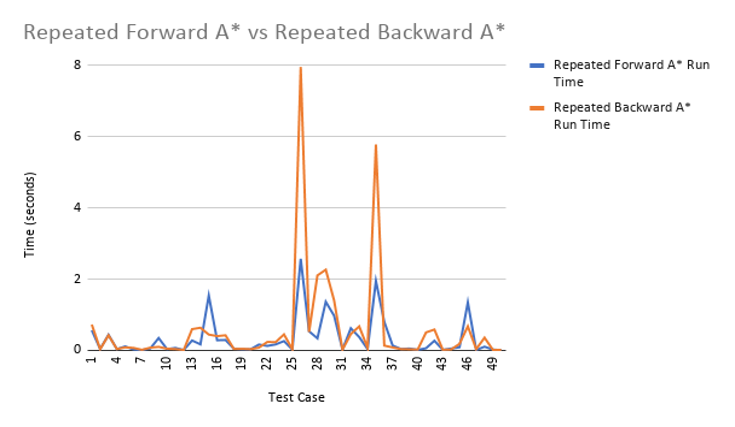
\includegraphics[width = 1\textwidth]{Part3_1.jpg} 
\end{center}
\caption{Comparing Repeated Forward A* and Repeated Backward A*}
\end{figure}

\paragraph{Explanation:}

When the blocked cells are more packed around the start state, forward A* is better then backward A*. Because once we get over the obstacle, we can go directly to the goal. The earlier we find the obstacle the better.

Same for the backward A*, when the blocked cells are more packed around the goal state, backward A* is better then forward A*. 

If we look at Figure 6 we can see an example of why Repeated Forward A* will work better when the blocked cells are closer to the start. When Repeated Forward A* is applied in a grid like this, it uncovers all blocked nodes at the beginning of the search, or more generally very early on in the search. This allows the agent to travel directly to the goal after all the blocked cells have been uncovered and it will not waste time expanding unnecessary nodes. On the other hand, the starting node is the goal node in Repeated Backward A* search. This means the Repeated Backward A* search will expand many unnecessary nodes, rather than nodes towards its goal, while it searches for the start node from the goal node.


\begin{figure}[h]
\begin{center}
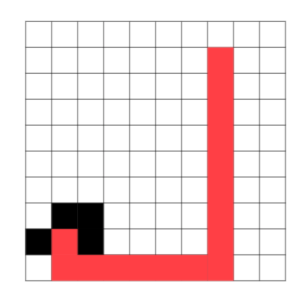
\includegraphics[scale=0.5]{Part3_2.png} 
\end{center}
\caption{Repeated Forward A*}
\end{figure}

\newpage

\section*{Part 4}
\paragraph{•}
The project argues that “the Manhattan distances are consistent in gridworlds in which the agent can move only in the four main compass directions.” Prove that this is indeed the case.\\

\textbf{Proof:}\\

We know a consistent heuristic is defined as:
$$h(n) \leq c(n, a, n')+h(n'), and\ h(x_G)=0$$ where h(n) is the estimated cost of reaching the goal from n, and $n'$ is the successor of n. $c(n, a, n')$ is the actual cost from n to $n'$.

Since we use Manhattan distance as h-value here, and the agent can only move in the four main compass directions, we use the index of row is denoted as X and the index of column is denoted as Y, then we can denote the Manhattan distance as:
$$h(s) = |X_s- X_{sgoal}| + |Y_s  - Y_{sgoal}|$$

(1) If S is the target state, which means $s = sgoal$ we can get:
$$h(sgoal) = |X_{sgoal} - X_{sgoal}| + |Y_{sgoal} - Y_{sgoal}| = 0$$
\hspace{20mm} Q.E.D.\\

\indent (2) If S is not the target state, we need to prove: $$h(s) – h(s’) \leq c(s, a, s’)$$
From the equation above we can get:
$$h(s) - h(s’) = (|X_s -X_{sgoal}| + |Y_s -Y_{sgoal}|) - (|X_{s’} -X_{sgoal}| + |Y_{s’} -Y_{sgoal}|)$$
Since the agent can only move to 4 compass directions and and only neighbor cells would be generated. Thus, s and $s’$ are neighboring cells in the grid. So it is either $X_s = X_{s’}$ or $Y_s = Y_{s’}$.\\

\indent \textbf{a)} If $X_s = X_{s’}$,
\begin{align*}
h(s) - h(s’) 
& =(|X_s -X_{sgoal}| + |Y_s -Y_{sgoal}|) - (|X_{s’} -X_{sgoal}| + |Y_{s’} -Y_{sgoal}|)  \\
& = |Y_s -Y_{sgoal}| - |Y_{s’} -Y_{sgoal}|
\end{align*}

\noindent By $|A| - |B| \leq |A-B|$, we can get:
\begin{align*}
h(s) - h(s’) 
& =|Y_s -Y_{sgoal}| - |Y_s -Y_{sgoal}|  \\
& \leq |(Y_s -Y_{sgoal}) - (Y_{s’} - Y_{sgoal})| = |Y_s - Y_{s’} | \\
\end{align*}
While $|Y_s - Y_{s’} | \leq 1 = c(s, a, s')$
$$h(s) - h(s’) \leq c(s, a, s')$$\\

\indent \textbf{b)} If $Y_s = Y_{s’}$,
\begin{align*}
h(s) - h(s’) 
& =(|X_s -X_{sgoal}| + |Y_s -Y_{sgoal}|) - (|X_{s’} -X_{sgoal}| + |Y_{s’} -Y_{sgoal}|)  \\
& = |X_s -X_{sgoal}| - |X_{s’} -X_{sgoal}|
\end{align*}

\noindent By $|A| - |B| \leq |A-B|$, we can get:
\begin{align*}
h(s) - h(s’) 
& =|X_s -X_{sgoal}| - |X_{s’} -X_{sgoal}| \\
& \leq |(X_s -X_{sgoal}) - (X_{s’} - X_{sgoal})| = |X_s - X_{s’} | \\
\end{align*}
While $|X_s - X_{s’} | \leq 1 = c(s, a, s')$
$$h(s) - h(s’) \leq c(s, a, s')$$
\hspace{20mm} Q.E.D.\\


\paragraph{•}
Furthermore, it is argued that “The h-values $h_{new}(s)$ ... are not only admissible but also consistent.” Prove that Adaptive A* leaves initially consistent h-values consistent even if action costs can increase.\\

\textbf{Proof:}\\

We know a consistent heuristic is defined as:
$$h(n) \leq c(n, a, n')+h(n'), and\ h(x_G)=0$$ where h(n) is the estimated cost of reaching the goal from n, and $n'$ is the successor of n. $c(n, a, n')$ is the actual cost from n to $n'$.

Now we have a new h-value defined as:$$h_{new}(s) = g(sgoal) - g(s)$$ where $g(sgoal)$ is the distance from the start state to the goal state of the previous path solution, $g(s)$ is the distance from the start state to the state s.

In adaptive A*, we only update the h-value of expanded nodes in the grid. So, we have three conditions here:\\

(1) Both $s$ and $s’$ have been expanded:\\

So the h-values of $s$ and $s'$ both need to be updated:
$$h_{new}(s ) = g(sgoal) - g(s)$$
$$h_{new}(s' ) = g(sgoal) - g(s')$$
in this case we need to prove that $h_{new}(s) \leq h_{new}(s') + c(s,a,s')  $.
Assume that:
 $$h_{new}(s) \leq h_{new}(s') + c(s,a,s')  $$
We substitute $h_{new}(s)$ and $h_{new}(s')$ in the equation above:

 $$g(sgoal) - g(s) \leq g(sgoal) - g(s') + c(s,a,s')  $$
 $$g(s')  \leq g(s) + c(s,a,s')  $$

$g(s’)$ is at most equals to $g(s) + c(n,a,n’)$ because $s’$ is the successor of s. But there are might also better solution path will be found later, so the parent of $s’$ might be a different node later, and the $s’$ would choose the parent that gives it the best g-value. At that time, since $s’$ is also expanded in this case, $s’$ must have the smallest g-value. Thus, $g(s’) < g(s) + c(n,a,n’)$.

We know that  $g(s')  \leq g(s) + c(s,a,s')  $ is true now. Thus, $h_{new}(s) \leq h_{new}(s') + c(s,a,s')  $ is also true.\\
\\

(2) $s$ had been expanded but $s'$ had not:\\

In this case, only the  h-value of $s$ would be updated:
$$h_{new}(s ) = g(sgoal) - g(s)$$
$$h(s') = h(s') \ (Manhattan\ distance)$$
Now we know from the case 1 that: 
\begin{equation} \label{eq:1}
g(s')  \leq g(s) + c(s,a,s')
\end{equation}
The f-value of a visited node in the previous A* search must be no smaller than any expanded node in the previous A* search, thus:
\begin{equation} \label{eq:2}
f(s) = g(s)+ h_{new}(s) \leq g(s’) + h(s’)
\end{equation}
We add (1) and (2) together:
$$g(s') + g(s)+ h_{new}(s) \leq g(s’) + h(s’) +g(s) + c(s,a,s')$$
$$h_{new}(s) \leq h(s’)  + c(s,a,s')$$\\


(3) Neither $s$ nor $s’$ had been expanded\\

Since neither $s$ nor $s’$ had been expanded, we would not update the h-value of them. Thus, the h-values of them are still Manhattan distance, which we proved consistent already.\\

\hspace{10mm} Q.E.D.\\

\newpage

\section*{Part 5}
Implement and compare Repeated Forward A* and Adaptive A* with respect to their runtime. Explain your observations in detail, that is, explain what you observed and give a reason for the observation. Both search algorithms should break ties among cells with the same f-value in favor of cells with larger g-values and remaining ties in an identical way, for example randomly.\\

\paragraph{Observation:}
From figure 7 we found that Repeated Forward A* with Adaptive A* is slightly faster than Repeated Forward A* for most of the cases, but the differences are not significant. 

\begin{figure}[h]
\begin{center}
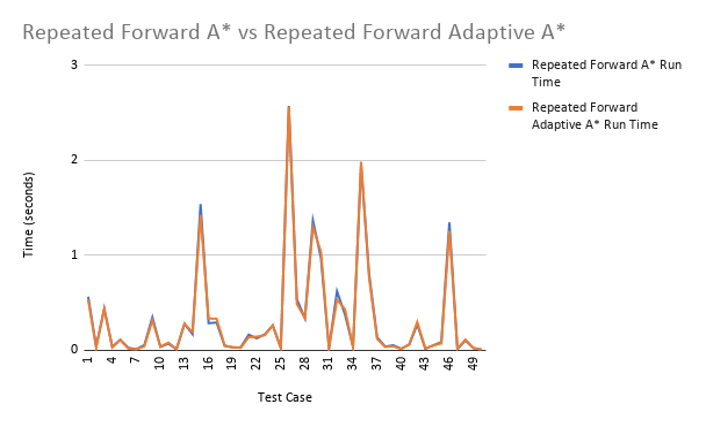
\includegraphics[width=1\textwidth]{Part5_1.jpg} 
\end{center}
\caption{Comparing Repeated Forward A* and Adaptive A*}
\end{figure}

\paragraph{Explanation:}
Comparing adaptive A* and forward A*, the adaptive A* would update h-value based on the knowledge from presumed shortest path, so that adaptive A* can prevent the agent has unnecessary moves.

The biggest difference between the two is that adaptive A* changes the h-value of the already expanded cells to a higher value, more accurate, consistent heuristic. This means that every time the A* algorithm computes a path the h-value heuristics becomes more accurate because the agent is learning as it moves along its path. Thus, adaptive A* can make better and more efficient choices as it repeats compared to normal A*. So the adaptive A* algorithm will generally expand less nodes than the normal A* algorithm.

Normally the adaptive A* algorithm does not come out to be too much faster because many of the nodes in a grid size of 101 x 101 are not expanded and adaptive A* only reevaluates the h-value for expanded nodes, meaning that much of the grid world remains unknown. On the other hand, after every A* search we must traverse the closed list and update all the h-values, which does take up a lot of time. This is another reason why adaptive A* is only slightly faster than regular A* algorithm.

However, the difference would be more significant in a real world scenario like a game-world, when the grid world is thousands of times larger than our 101*101 grid, it might be far faster if using adaptive.


\newpage

\section*{Part 6}
You performed all experiments in gridworlds of size 101 × 101 but some real-time computer games use maps whose number of cells is up to two orders of magnitude larger than that. It is then especially important to limit the amount of information that is stored per cell. For example, the tree-pointers can be implemented with only two bits per cell. Suggest additional ways to reduce the memory consumption of your implementations further. Then, calculate the amount of memory that they need to operate on gridworlds of size 1001 × 1001 and the largest gridworld that they can operate on within a memory limit of 4 MBytes.\\

\paragraph{Answer:}
In order to reduce the memory usage, we could improve the way that we stored the cell  and grid information. In order to make our base grids, we created a binary array using the numpy package. As a default, this stores the array values as int-32. However, because we knew that our array would only ever hold 1's and 0's, we were able to specifiy that the numpy array should store as int-8. This one change allowed us to cut the amount of storage needed per maze by 1/4. Although this is not a large savings for grid worlds of size 101 * 101, in real world environments, this could be a huge savings

In the implementation, we store the node as a cell, each cell contains \{f-value, g-value, h-value, location, parent\}. We store f-value, g-value, and h-value as an integer, we store location as a tuple, the parent is also denoted as a tuple, which is the location of the parent.

Assume that we are using C and we will use C sizes in bytes in the analysis as below, since in python the data types are objects and sizes vary with how much is stored in each variable.

Say we use 4 bytes to store each f-value, g-value and h-value, and since we use 2 integers to represent location, we use 8 bytes to store location of current node and 8 bytes to store the parent of current node.

Such that each cell takes 4+4+4+8+8 = 28 bytes\\

However, we can improve it by representing the parent information by something else. Since the parent of the current node will only from the four compass directions, we can use 2 bits, [00, 01, 10, 11] to represent the four compass directions. Such that we can store the direction in cell as the information of the parent. \\

1 byte = 8 bits, 1 bit = 0.125 byte, we use 2 bits to store the direction\\

Now, each cell takes 4+4+4+8+0.25 = 20.25 bytes\\

In the grid world of size 1001* 1001 the worst case, we need to store the whole grid in expanded list within one A* search,

$$1001 \times 1001 \times 20.25 = 20290520.25 \ bytes = 20.29052025 \ MB$$

For 4 MB limit, they can operate on:\\

4MB = 4000000 bytes\\

Grid size = $\sqrt{4000000/20.25} = 444$\\

So the grid will be $444 \times 444$



\end{document}
